\chapter{Resultados}\label{chap:results}

\section{Regras de associação}

Para esta análise as funções que o R oferece não são suficientes pelo que foi necessário instalar um \textit{package} adicional, \textit{arules}, que oferece uma vasta quantidade de funções direcionadas para regras de associação. Ao contrário das secções anteriores, nesta secção usam-se os vários parâmatros com os seus valores já discretizados, para que o algoritmo utilizado seja mais eficiente. O processo de de procura de regras de associação é de fácil compreensão: o algoritmo vai percorrer o \textit{data set} e analisar cada ``transação'', que corresponde a cada linha do ficheiro csv. Dependendo da confiança e suporte escolhidos, vai gerar algumas regras que conseguir encontrar e que respeitem os limites escolhidos. As regras geradas podem ser de qualquer tipo, isto é, o consequente pode ser qualquer uma das variáveis analisadas, sendo que neste caso interessa-nos descobrir regras com a variável ``Value\textunderscore Glucose'' como consequente, ou seja, no lado direito. Contudo, o \textit{data set} ainda não está estruturado da melhor forma para a criação das regras. 
Da forma que o \textit{data set} está feito, cada linha corresponde ao mesmo momento, ou seja, se uma linha tiver um valor de glicemia, hidratos de carbono e insulina, tudo isso corresponde a um registo feito à mesma hora. O mesmo acontece para o exercício. O tipo de conclusões que se pretende obter é de que forma estes parâmetros causam algum impacto no valor de glicemia, como por exemplo, descobrir de que forma o exercício vai alterar a quantidade de glucose no sangue ou de que forma a insulina tomada ou os hidratos de carbono vão fazer alterar este valor. Se todos esses parâmetros forem registados à mesma hora, não se consegue concluir nada: uma vez que o algoritmo Apriori vai analisar linha a linha de forma independente, no formato atual, o valor de glicemia só vai ser comparado com o valor de insulina e de hidratos de carbono registados ao mesmo tempo. No entanto, o importante é saber como é que a quantidade de hidratos de carbono ingerida e a insulina tomada vão afetar a glicemia no espaço de tempo a seguir, e não no mesmo espaço de tempo. Ou seja, como é que os valores de hidratos e de insulina num registo, vão afetar a glicemia no registo seguinte. A questão é que o valor de glicemia do registo seguinte vai pertencer a outra linha do csv e portanto não vai ser tido em conta para os valores de outra linha. Posto isto, a solução foi alterar a estrutura do ficheiro para que cada linha passe a ter o valor de glicemia seguinte, e não o atual. Assim, imaginando que a variável ``Value\textunderscore Glucose'' passe a chamar-se ``Next\textunderscore Glucose'', é possível ter uma regra como

\begin{lstlisting}
Se Value_Carbs==5 entao Next_Glucose==5
\end{lstlisting} 

ou seja, descobrir um padrão em que quando o utilizador ingere demasiados hidratos de carbono, então o valor seguinte de glicemia será demasiado elevado, mais precisamente uma hiperglicemia. Se esta alteração não fosse feita, as regras descobertas apenas dariam relações entre valores registados à mesma hora o que não tem qualquer utilidade. Embora este não seja o único tipo de regras a descobrir, certamente que é um dos tipos de conselhos que podem levar um utilizador a conseguir controlar a diabetes de forma mais eficiente. Convém relembrar que se uma regra é descoberta, é porque essa ação ocorre várias vezes, ou seja, trata-se de um padrão. Ao informar o utilizador de que este padrão existe, e que tem uma influência negativa nos seus valores de glicemia, o utilizador pode tomar a ação que achar mais apropriada de forma a evitar que aconteça. Na presença de uma regra como esta, a aplicação poderia mostrar um aviso quando o utilizador fosse fazer um registo de refeição e metesse um valor elevado de hidratos de carbono, em que o aviso poderia ser, por exemplo, ``Meteu um valor de hidratos de carbono elevado e, quando faz isso, normalmente tende a ter uma eventual hiperglicemia algum tempo depois da refeição''.

Uma vez alterados os \textit{data sets} de cada utilizador, faltava ainda converter todas as variáveis para \textit{factor}. \textit{Factor} é um tipo em R que toma apenas um número limitado de valores diferentes; variáveis do tipo \textit{factor} são também chamadas de variáveis categóricas. Esta conversão é necessária para as variáveis poderem ser utilizadas no algoritmo de associação. Ainda assim, a fase de discretização feita na secção 5.2 é também necessária. Sem a discretização, as variáveis podem ser utilizadas pelo apriori desde que sejam do tipo \textit{factor} mas as regras geradas não são utilizáveis. Por exemplo, uma regra gerada sem fazer discretização das variáveis é

\begin{lstlisting}
{Value_Glucose=140,Value_Insulin=140} => {Value_Carbs=140}
\end{lstlisting}

que serve para ilustrar a ineficácia deste algoritmo para valores não discretizados. Feito então o passo de conversão das variáveis para \textit{factors}, o \textit{data set} está pronto a ser utilizado pelo apriori. De seguida apresentaremos algumas das regras mais relevantes descobertas para cada utilizador e verificaremos também se essas regras estão em concordância com os gráficos obtidos na secção anterior. Todas as regras terão uma confiança mínima de 60\%.
Para cada utilizador interessa-nos descobrir regras que levem a alterações do valor de glicemia, sendo que o valor normal, tal como definido na secção 5.1, é 3. Portanto, interessa descobrir regras em que o valor de glicose seja 1 ou 2 para valores baixos e 4 ou 5 para valores altos.

O algoritmo \textit{apriori} vai analisar linha a linha dos dados e tentar descobrir relações entre as variáveis. Para obter as regras cujo consequente diga respeito aos valores anormais de glicemias, é preciso filtrar as regras geradas. Neste caso, vamos filtrar o conjunto de regras de forma a mostrar apenas regras com ``Next\textunderscore Glucose'' com valores 1, 2, 4 ou 5. 

Para todos os utilizadores definimos uma confiança mínima de 0.6 e um suporte mínimo de 0.01. O suporte tem que ser bastante baixo uma vez que vamos aplicar o algoritmo num \textit{data set} pequeno. Isto porque estamos à procura de padrões que, embora recorrentes, vão ser uma minoria dos dados. Naturalmente que num \textit{data set} com milhares de linhas esses padrões são mais óbvios, ou seja, mais frequentes, e portanto um suporte mais alto seja suficiente para encontrar. Por outro lado, para \textit{data sets} com dezenas ou poucas centenas de linhas, os padrões não são tão explícitos pelo que é necessário um suporte mais baixo para descobrir regras. Usar um suporte demasiado baixo pode fazer com que sejam descobertas regras que sejam um caso pontual, pelo que convém não usar um suporte demasiado baixo. Assim, foi escolhido o valor 0.01 que é um valor baixo mas não demasiado. 

Para a confiança foi escolhido o valor mínimo de 0.6 o que significa que, para cada regra, se o antecedente acontece, então o consequente irá acontecer com 60\% de probabilidade, o que confere alguma segurança às regras. As regras que cumpram estes dois requisitos são chamadas de regras fortes.


No R, o comando para a geração de regras através do algoritmo \textit{apriori} é

\begin{lstlisting}
rules <- apriori(dataset, parameter=list(confidence=0.6, support=0.01))
\end{lstlisting}

em que ``dataset'' é o ficheiro a ser analisado com os parâmetros confiança e suporte definidos com os valores já mencionados. Para mostrar apenas as regras com o valor de glicose pretendido, como por exemplo 5, o comando é

\begin{lstlisting}
rules.sub <- subset(rules, subset = rhs %in% "Next_Glucose=5")
\end{lstlisting}

que gerará então um subconjunto de regras em que o consequente será ``Next\textunderscore Glucose=5''.

Existe um \textit{package} chamado \textit{arulesViz} que é uma ferramenta para visualizar as regras geradas. Este \textit{package} permite, por exemplo, ordenar as regras geradas por confiança ou \textit{lift} e assim filtrar quais as regras potencialmente mais úteis. Isto é feito de forma interativa: no gráfico é possível selecionar uma região com regras e todas as regras existentes nessa região serão mostradas.
De seguida, apresentaremos algumas regras geradas para cada utilizador.

\textbf{Utilizador 1}

Para o utilizador foram geradas 1239 regras. Obviamente que se torna impossível de analisar todas as regras individualmente, pelo que o primeiro passo será então aplicar um filtro, de forma a ficar apenas com valores anormais de glicemia no consequente. Após este filtro, o conjunto de regras diminui bastante, para 25. Com o comando

\begin{lstlisting}
plot(rules.sub, method=NULL, measure="support", shading = "lift", interactive = TRUE, data = NULL, control = NULL)
\end{lstlisting}

obtém-se o gráfico

\begin{figure}[H]
\centering
\includegraphics[scale=0.5]{/home/tiago/Tese/Tese/Databases/CSV/Data/ImagensTese/Utilizador1/Regras.pdf}
\caption{Glicemia por horas do utilizador 5}
\end{figure}

e escolhe-se a região no canto inferior esquerdo, que o suporte mais elevado. Essa região contém a regra

\begin{lstlisting}
{Day=Quarta,Period=2,Value_Carbs=4} => {Next_Glucose=4}

\end{lstlisting}

Por outro lado, as regras geradas para valores baixos de glicose são

\begin{lstlisting}
{Day=Sexta,Period=1,Value_Carbs=3} => {Next_Glucose=2}
\end{lstlisting}

que mostra que à sexta-feira de manhã o utilizador tende a ter valores mais baixos que nos outros dias.


\textbf{Utilizador 2}

Para o utilizador 2 é expectável que se consigam mais regras do que para o utilizador 1 visto que o utilizador 2 tinha valores de glicemia mais oscilatórios. 


\begin{figure}[H]
\centering
\includegraphics[scale=0.5]{/home/tiago/Tese/Tese/Databases/CSV/Data/ImagensTese/Utilizador2/Regras.pdf}
\caption{Glicemia por horas do utilizador 5}
\end{figure}


\begin{lstlisting}


{Day=Quinta,Period=2}     => {Next_Glucose=5} 0.0499002 0.625      1.527439
{Day=Sexta,Period=2} => {Next_Glucose=5}

\end{lstlisting}

Enquanto que para o primeiro utilizador não se descobriram regras para valores de glicose 5, para este já se descobriu, por exemplo, que às quartas-feiras o utilizador tende a tomar pouca insulina o que reflete um valor bastante alto de insulina. Por sua vez, às quintas-feiras durante a tarde os valores também costumam ser demasiado elevados. 






\textbf{Utilizador 3}

Para este utilizador, para ``Next\textunderscore Glucose=5'' foram geradas 150 regras, tornando-se por isso necessário filtrar algumas, usando gráficos, uma vez mais. 


\begin{figure}[H]
\centering
\includegraphics[scale=0.5]{/home/tiago/Tese/Tese/Databases/CSV/Data/ImagensTese/Utilizador3/Regras.pdf}
\caption{Glicemia por horas do utilizador 5}
\end{figure}

Como se pode ver pela figura, selecionámos a região que engloba as regras com maior suporte. Uma vez que temos poucos dados, torna-se mais difícil avaliar a importância das regras. Por exemplo, as regras com maior \textit{lift} são as regras com menor suporte, o que aumenta o risco de serem situações pontuais e não recorrentes. Por outro lado, as regras com maior suporte têm menor \textit{lift}, embora seja superior a 1. Num \textit{data set} com mais dados, talvez a escolha recaísse sobre as regras com maior \textit{lift} mas, para garantir o máximo possível que as regras correspondem a situações repetidas, optamos por mostrar algumas das regras com maior suporte, ou seja, na região mais escura. Algumas dessas regras são:

\begin{lstlisting}
{Period=2, Value_Carbs=4}       => {Next_Glucose=5} 0.07284768  0.9166667 2.162760  
{Period=3, Value_Insulin=3}     => {Next_Glucose=5} 0.09933775  0.6521739 1.538723
{Value_Carbs=4} => {Next_Glucose=5} 0.07947020  0.8000000 1.887500
\end{lstlisting}

Será também interessante, no entanto, ver algumas das regras com maior \textit{lift}, que são

\begin{lstlisting}
{Day=Terca,Period=2} => {Next_Glucose=5} 0.0397351 1          2.359375
\end{lstlisting}

que corresponde à parte superior do gráfico, sendo esta a regra mais à direita (ou seja, maior suporte). 

Para valores de glicemia baixos, não são geradas quaisquer regras, o que seria de esperar, pois pela figura x pode-se verificar que o utilizador tem poucos valores de glicemia próximos do limite de hipoglicemia, pelo que serão ocorrências pontuais. 


\textbf{Utilizador 4}

Para este utilizador foram geradas 41 regras para valores de hiperglicemia.



\begin{figure}[H]
\centering
\includegraphics[scale=0.5]{/home/tiago/Tese/Tese/Databases/CSV/Data/ImagensTese/Utilizador4/Regras.pdf}
\caption{Glicemia por horas do utilizador 5}
\end{figure}
 A zona sombreada no gráfico corresponde às regras com maior suporte,
 

\begin{lstlisting}

{Day=Sexta, Value_Insulin=3, Insulin_Difference=4} => {Next_Glucose=5} 0.03355705      0.625 2.217262

\end{lstlisting}

Algumas das regras com maior \textit{lift}, embora com um suporte consideravelmente mais pequeno, são

\begin{lstlisting}
{Day=Terca, Value_Carbs=5, Insulin_Difference=2} => {Next_Glucose=5} 0.01342282          1 3.547619
{Day=Sabado, Period=3, Value_Carbs=3}    => {Next_Glucose=5} 0.01342282          1 3.547619
\end{lstlisting}



\textbf{Utilizador 5}

Também para este utilizador utilizaremos a ferramenta visual para ajudar a escolher as regras mais úteis, pois são geradas 136 regras para valores de hiperglicemia. 

\begin{figure}[H]
\centering
\includegraphics[scale=0.5]{/home/tiago/Tese/Tese/Databases/CSV/Data/ImagensTese/Utilizador5/Regras.pdf}
\caption{Glicemia por horas do utilizador 5}
\end{figure}


\begin{lstlisting}
{Period=2,Value_Insulin=3} => {Next_Glucose=5} 0.09615385 0.625      1.477273 3    
{Period=2,Value_Carbs=3} => {Next_Glucose=5} 0.09615385 0.625      1.477273 3    
\end{lstlisting}

Este utilizador tem tendência para hiperglicemias durante o período da tarde, mesmo que consuma hidratos de carbono numa quantidade normal ou tome um valor de insulina moderado. Isto pode significar que o utilizador, ao almoço por exemplo, não faz uma contagem de hidratos correta ou não adeque a insulina pelo que causa valores mais elevados durante a tarde. 

\section{Redes \textit{Bayesianas}}

Nesta secção iremos criar uma rede \textit{bayesiana} para cada um dos utilizadores, de forma a perceber de que forma as regras geradas na secção anterior influenciam o valor de glicemia. Por exemplo, se um dado utilizador tiver uma regra que diga que à quarta-feira à tarde costuma ter hiperglicemias, qual será, então, a probabilidade de ter uma hiperglicemia numa quarta-feira à tarde? Uma rede \textit{bayesiana} permite isto ao calcular as probabilidades de cada variável tomar um determinado valor. Portanto, uma rede feita a partir do mesmo \textit{data set} que as regras de associação, deverá estar em concordância com essas regras. Mas mais que isso, dá informação extra sobre como é que as várias variáveis influenciam a variável de interesse, que para este trabalho é o valor de glicemia.

O primeiro passo nesta fase é então criar uma rede \textit{bayesiana}, recorrendo ao \textit{software} WEKA. Antes de mais, é preciso preparar o \textit{data set} para ser utilizado pelo WEKA, que será igual ao utilizado para as regras de associação mas com o detalhe que a variável ``Next\textunderscore Glucose'' terá de ser a última variável do ficheiro, ou seja, a coluna mais à direita. Isto faz com que o WEKA a considere como a variável de classe, ou seja, a variável a prever e, portanto, o \textit{data set} está pronto a ser usado pelo WEKA. Note-se que o WEKA vai ser utilizado apenas para criar a rede \textit{bayesiana}, que será analisada pelo SamIAm.

O comando utilizado para criar a rede é

\begin{lstlisting}
java -cp weka.jar weka.classifiers.meta.FilteredClassifier -t dataset.csv -T dataset.csv -distribution -p 0 -threshold-label  -threshold-file datasetThreshold.arff -d weka.tan2.model -i  -W weka.classifiers.bayes.BayesNet -- -D -Q weka.classifiers.bayes.net.search.local.TAN -- -S BAYES -E weka.classifiers.bayes.net.estimate.SimpleEstimator -- -A 0.000001 


java -cp weka.jar weka.classifiers.meta.FilteredClassifier -l weka.tan2.model -T dataset.csv -g > weka_tan2.xml

\end{lstlisting}

que, como se pode verificar, tem vários parâmetros.

O parâmetro -t é o ficheiro de treino e -T diz respeito ao ficheiro de teste.
-d é o ficheiro \textit{output} do modelo;
-i dá um \textit{output} detalhado sobre informação estatística para cada classe;
-W dá o nome completo do classificador
-D especifica para não usar ADTree, pois não é útil para \textit{data sets} pequenos
-Q especifica o algoritmo de procura
-E especifica o algoritmo de estima em que \textit{SimpleEstimator} é usado para estimar as tabelas de probabilidade condicional na rede

Este comando gera a rede


\begin{figure}[H]
\centering
\includegraphics[scale=0.7]{/home/tiago/Tese/Tese/Databases/CSV/Data/ImagensTese/Rede.png}
\caption{Glicemia por horas do utilizador 5}
\end{figure}


O SamIAm tem dois modos disponíveis: \textit{Edit mode} e \textit{Query mode} sendo que vamos utilizar o programa em \textit{Query mode}. 

A figura anterior mostra a rede \textit{bayesiana} criada pelo WEKA com o SamIAm em \textit{Edit mode}. Este modo serve para alterar a estrutura da rede, como adicionar nós ou arestas, mas não é esse o nosso objetivo. O objetivo é, uma vez mais, perceber de que forma as variáveis se relacionam, ou seja, como é que a alteração de uma variável provoca alterações noutra variável. Nesse caso, torna-se útil usar o \textit{query mode}. 

Este modo permite ver a probabilidade de cada variável tomar cada valor, de acordo com o \textit{data set} e permite também mudar esses valores e ver de que forma as outras variáveis mudam também. Por exemplo, uma regra possível seria ``Um utilizador tem tendência para ter valores de glicemia altos à quarta-feira à tarde''. É interessante e útil para o utilizador conhecer esta regra, por si só. Mas também pode ser interessante o processo inverso, ou seja, ``Qual a probabilidade de ter hiperglicemia, sendo que hoje é quarta-feira à tarde?''. É isso que o SamIAm permite fazer no \textit{query mode}, entre outras coisas, e que pode dar mais informação útil ao utilizador. A figura seguinte mostra a mesma rede mas em \textit{query mode}.

\begin{figure}[H]
\centering
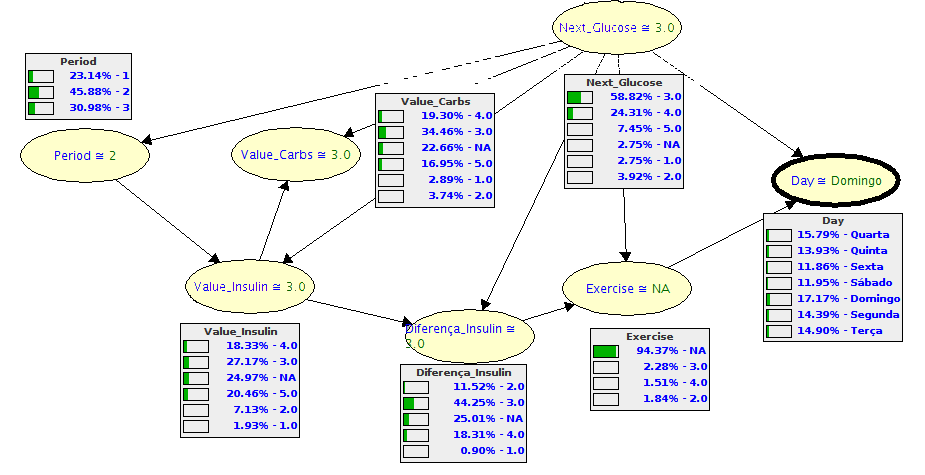
\includegraphics[height=65mm, width=130mm]{/home/tiago/Tese/Tese/Databases/CSV/Data/ImagensTese/Utilizador1/Sam.png}
\caption{Glicemia por horas do utilizador 5}
\end{figure}

É possível ver as tabelas de probabilidade para cada variável, sendo que cada nó tem por predefinição o valor mais frequente, como por exemplo, ``Next\textunderscore Glucose=3''. Note-se que os valores NA correspondem a registos que não usaram essas variáveis, isso é, um utilizador pode registar uma glicemia e não registar insulina ou hidratos d carbono. Estas tabelas também permitem perceber a distribuição de algumas variáveis: por exemplo, é possível verificar que, neste caso, os dias têm probabilidades muito parecidas, o que significa que têm um número parecido de registos. No entanto, tal como já mencionado, o objetivo nesta parte é tentar perceber de que forma estas variáveis afetam o valor da glicemia e também ver se estas alterações estão em concordância com as regras mostradas na secção anterior ou até ver se novos padrões surgem. Vamos, por isso, mostrar a rede \textit{bayesiana} para cada utilizador. 

\textbf{Utilizador 1}

Para este utilizador, a tabela de probabilidades inicial é mostrada na figura

\begin{figure}[H]
\centering
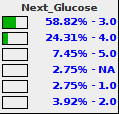
\includegraphics{/home/tiago/Tese/Tese/Databases/CSV/Data/ImagensTese/Utilizador1/Probs.png}
\caption{Glicemia por horas do utilizador 5}
\end{figure}

uma das regras geradas mostrava que, às quartas-feiras à tarde e quando o utilizador ingere hidratos de carbono em valores elevados, a glicemia tomava valores elevados. Ao selecionar, então, no SamIAm, esses três parâmetros com os valores definidos na regra, verifica-se que a probabilidade de ``Next\textunderscore Value=4'' sobe para 62.68\%.

Por outro lado, se colocarmos as variáveis de acordo com a regra para hipoglicemia neste utilizador, verificamos que a probabilidade de ``Next\textunderscore Glucose=2'' sobe para 34.74\%.

No entanto, é possível descobrir outros padrões: por exemplo, se selecionarmos apenas o dia ``Domingo'' verificamos que a probabilidade de uma hiperglicemia, ou seja um valor de glicemia 5, sobe para 18.67\%. 

Na figura seguinte pode-se ver quais os parâmetros que provocam uma probabilidade máxima de uma hiperglicemia.

\begin{figure}[H]
\centering
\includegraphics[height=65mm, width=130mm]{/home/tiago/Tese/Tese/Databases/CSV/Data/ImagensTese/Utilizador1/Hiper.png}
\caption{Glicemia por horas do utilizador 5}
\end{figure}

Ou seja, uma nova regra é descoberta: ao Domingo de manhã, quando o utilizador ingere uma quantidade grande de hidratos de carbono, tem maior probabilidade de ter uma hiperglicemia. 

\textbf{Utilizador 2}


A rede para o utilizador 2 é mostrada na figura seguinte

\begin{figure}[H]
\centering
\includegraphics[height=65mm, width=130mm]{/home/tiago/Tese/Tese/Databases/CSV/Data/ImagensTese/Utilizador2/Rede.png}
\caption{Glicemia por horas do utilizador 5}
\end{figure}

que, como se verifica, é ligeiramente diferente da rede gerada para o utilizador 1. Uma vez mais, é interessante ver quais os valores dos vários parâmetros que maximizam o valor de glicemia. 

\begin{figure}[H]
\centering
\includegraphics[height=65mm, width=130mm]{/home/tiago/Tese/Tese/Databases/CSV/Data/ImagensTese/Utilizador2/Hiper.png}
\caption{Glicemia por horas do utilizador 5}
\end{figure}

Como se pode observar, a probabilidade de hiperglicemia aumenta bastante aos sábados à tarde, quando o utilizador toma menos insulina que a recomendada. Esta regra não foi gerada pelo algoritmo \textit{apriori}, possivelmente por ter um valor de suporte abaixo do mínimo definido, mas ainda assim é uma regra interessante e que mostra uma utilidade desta análise. É interessante saber quais as condições em que o risco de hiperglicemia é maior, tendo em conta os dados já registados. 

\textbf{Utilizador 3}

A rede criada para o utilizador 3 está representada na figura

\begin{figure}[H]
\centering
\includegraphics[height=65mm, width=130mm]{/home/tiago/Tese/Tese/Databases/CSV/Data/ImagensTese/Utilizador3/Rede.png}
\caption{Glicemia por horas do utilizador 5}
\end{figure}

que é diferente das redes dos utilizadores anteriores, principalmente pelo facto de este utilizador não ter qualquer registo de exercício, pelo que essa variável não foi tida em conta.

\begin{figure}[H]
\centering
\includegraphics[height=65mm, width=130mm]{/home/tiago/Tese/Tese/Databases/CSV/Data/ImagensTese/Utilizador3/Hiper.png}
\caption{Glicemia por horas do utilizador 5}
\end{figure}

Como se pode ver na figura anterior, este utilizador tem uma probabilidade enorme de ter hiperglicemia à terça-feira à tarde, especialmente se tomar menos insulina que a calculada. 

\textbf{Utilizador 4}

A rede \textit{bayesiana} para o utilizador 4 está representada na figura seguinte.

\begin{figure}[H]
\centering
\includegraphics[height=65mm, width=130mm]{/home/tiago/Tese/Tese/Databases/CSV/Data/ImagensTese/Utilizador4/Rede.png}
\caption{Glicemia por horas do utilizador 5}
\end{figure}

e alterando alguns valores, obtém-se um exemplo em que a probabilidade de hiperglicemia é aumentada, como se pode perceber pela figura.

\begin{figure}[H]
\centering
\includegraphics[height=65mm, width=130mm]{/home/tiago/Tese/Tese/Databases/CSV/Data/ImagensTese/Utilizador4/Hiper.png}
\caption{Glicemia por horas do utilizador 5}
\end{figure}

Verifica-se que a probabilidade de o utilizador ter uma hiperglicemia é consideravelmente maior à segunda-feira que a qualquer outro dia, sendo que os outros parâmetros têm, neste caso, pouca influência, ou seja, a probabilidade de ter hiperglicemia à segunda-feira é praticamente igual para todos os períodos, por exemplo.

Por outro lado, verificamos que o utilizador tem uma maior probabilidade de ter um valor de hipoglicemia, isto é, ``Next\textunderscore Glucose=1'' à sexta-feira à tarde, cuja probabilidade aumenta para os 10.19\%.


\textbf{Utilizador 5}


Para o último utilizador, a rede gerada está representada na figura

\begin{figure}[H]
\centering
\includegraphics[height=65mm, width=130mm]{/home/tiago/Tese/Tese/Databases/CSV/Data/ImagensTese/Utilizador5/Rede.png}
\caption{Glicemia por horas do utilizador 5}
\end{figure}

Uma vez mais, um exemplo de uma combinação de parâmetros que aumentam a probabilidade de hiperglicemia, representada na figura seguinte.

\begin{figure}[H]
\centering
\includegraphics[height=65mm, width=130mm]{/home/tiago/Tese/Tese/Databases/CSV/Data/ImagensTese/Utilizador5/Hiper.png}
\caption{Glicemia por horas do utilizador 5}
\end{figure}

que mostra que à segunda-feira, e quando o utilizador toma menos insulina que a recomendada, os valores de glicose aumentam. 

Por outro lado, vemos que a probabilidade de ``Next\textunderscore Glucose=1'' nas manhãs em que o utilizador toma mais insulina que aquela recomendada, sendo que neste caso a probabilidade é de 20.09\%.



